\section{Comm. Basics}
\redtext{ISO OSI:}
Open Systems Interconnection model, 
Basis for standards development on SY interconnection,
Reference model.
\textbar
\redtext{Layers:}
\bluetext{
Application(Peer protocol: HTTP, DNS, FTP);
Presentation;
Session;
Transport: TCP/UDP;
Network: IP;
Data link;
Physical}
\\ 
\redtext{IPv4 v6(no checksum):}
Relays datagrams accross networks,
Routing enables internetworking,
Deliver packet from source to host address,
Foundation for TCP/UDP
\\
\redtext{IP routing:}routing protocol,
\bluetext{BGP} used in internet:
Border Gateway Protocol,
Routing between AS (Autonomous systems, provider or bigger organization),
Exchanges routing and reachability information between AS.
\\
\redtext{TCP:} for \bluetext{HTTP, RPC},
Slower than UDP, but with reliability using ACK,
Connection oriented protocol, session is initiated,
Provides ordering, sequencing,
Flow control, sender can't overflow receiver(same speed sending, receiving),
PortNum in TCP protocol(not in IP protocol)
\\
\redtext{UDP:} for \bluetext{DNS, Video, Voice},
Faster than TCP,
Connectionless(no session);
Best-effort;
Packet independent; 
No guaranteed delivery;
No ordering guarantees;
P2P and P2-multipoint.
\\
\redtext{Ports:}
a 16 bit number to local host to identify the connection, 
to differentiate APPs, if packet arrive;
Separate for \bluetext{UDP and TCP};
$0-1023$ reserved to root,
$1024 - 65535$  available to regular user;
http 80/tcp, ftp 21/tcp, ssh 22/tcp, telnet 23/tcp, finger 79/tcp, snmp 161/udp
\\
\redtext{APP Layer protocol:}
Set of rules specifying data transfer
between computing end-points
(Connection establishment \& tear-down
Data representation,
Comm);
\bluetext{DHCP} (Dynamic Host Configuration Protocol),
\bluetext{HTTP} (Hypertext Transfer Protocol),
\bluetext{FTP} (File Transfer Protocol),
\bluetext{Telnet} (Telnet Remote Protocol),
\bluetext{SSH} (Secure Shell Remote Protocol),
\bluetext{SIP} (Session Initiation Protocol),
\bluetext{POP3} (Post Office Protocol 3),
\bluetext{SMTP} (Simple Mail Transfer Protocol),
\bluetext{IMAP} (Internet Message Access Protocol),
\textbar \textbar
browser retreives web page(HTTP 1.1 over TCP, HTTP, FTP, SMTP)
\\
\redtext{HTTP/1.0 C S:}
\bluetext{Request}: GET <path>/index.html HTTP/1.0
\bluetext{Response}: HTTP/1.0 200 OK
\bluetext{ErrorResponse}: HTTP/1.0 404 Not Found 
\textbar \textbar
\redtext{HTTP/1.1:}
HyperText Transfer Protocol,
Request/Response protocol for C S comm. on top of TCP
(Browser,
RESTFUL API‘s,
SOAP over HTTP,
NoSQL databases)
\bluetext{Methods:}
\bluetext{GET:}cacheable get info by Request-URI
\bluetext{HEAD:} like GET but MUST NOT return a message-body
\bluetext{POST:} post a form (bulletin board), uploading data,
can be a data-accepting process
Responses not cacheable(200 (OK), 204(No Content), 201
(Created), 303 (See Other)) 
\bluetext{PUT:} Enclosed entity to be stored under Request-URI
Responses not cacheable
\bluetext{DELETE:} Delete the resource by Request-URI
Response: 200 (OK), 202 (Accepted), 204 (No Content)
\bluetext{TRACE:} for diagnostics
\bluetext{CONNECT:} to initialize secure connection, HTTPS on port 443,
Proxy is asked to forward the TCP connection
\textbar
\redtext{HTTP/1.1 proxy:}C \bluetext{GET req.} $\rightarrow$ Proxy, but not in cache. 
Proxy \bluetext{GET req.} $\rightarrow$ Origin, Origin $\rightarrow$ Proxy response.
C \bluetext{GET req.} $\rightarrow$ Proxy, Proxy $\rightarrow$ C cached resp.
\textbar
\redtext{HTTP/2.0:}
Better utilization network capacity,
Headers compressed,
On a single connection req and resp interleaved,
Prioritization of requests
% FIXME: can be removed
GET/HTTP/1.1
Host:www.tum.de
Connection:keep-alive
Accept: text/html,application/xhtml+xml,application/xml;q=0.9, image/webp, */*;q=0.8
User-Agent: Mozilla/5.0 (X11; Linux x86\_64) AppleWebKit/537.36 (KHTML, like Gecko) Chrome/37.0.2062.120 Safari/537.36
Accept-Encoding: gzip,deflate,sdch
\textbar \textbar \textbar
HTTP/1.1 200 OK
Date: Wed, 08 Oct 2014 15:25:53 GMT
Server: Apache
X-Powered-By: PHP/5.5.17
Content-Encoding: gzip
%
%
%
\subsection*{Socket}
Move data/Msg/(invoke operation/service and return result/failure) 
from APP I on Host A to APP K on Host B.
\rtext{Client}:Issues requests to server(send \& receive).
\rtext{Server}:Starts up and listens for connections, requests, and sends/receives.
\rtext{Client/Server examples}: telnet/telnetd, ftp/ftpd (sftp/sftpd), Firefox/Apache.
\rtext{Socket}: network programming abstraction for communicating among processes (applications) based on (Unix) file
descriptors.
\rtext{File descriptor}:an integer representing an open file managed by the OS \textbackslash In Unix any I/O is done by reading/writing from/to file
descriptors.
\rtext{Socket types}: 
Stream socket:java.net.ServerSocket, TCP based, Ordering guaranteed, Error-free 
\textbackslash Datagram socket:java.net.DatagramSocket, UDP based 
\textbackslash IPv4 \& IPv6

% TODO: add this pic surrowed by words
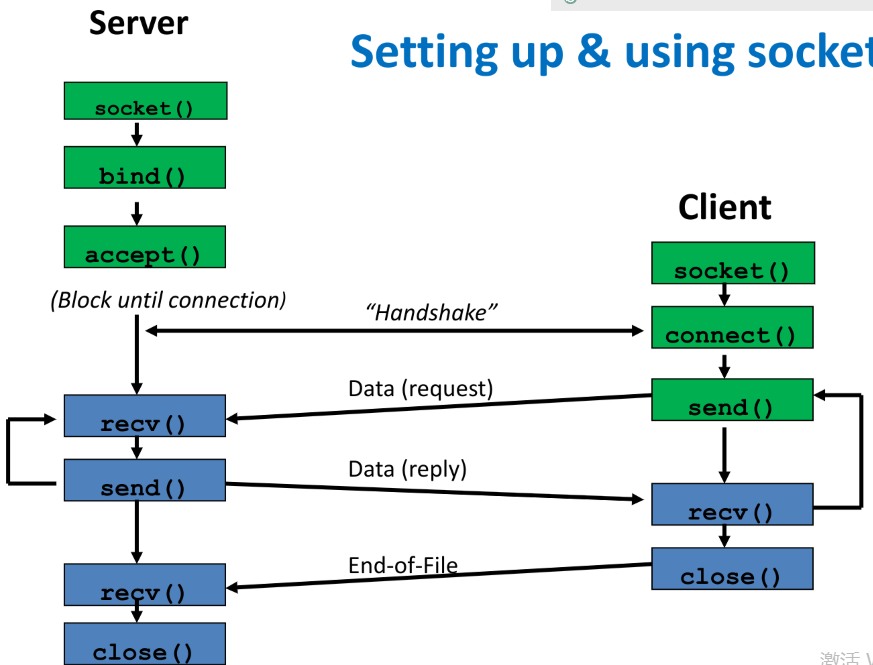
\includegraphics[width=.8\linewidth]{chap1_1.png}
\subsection*{NIO(Nonblocking sockets)}
\rtext{Synchronous}: Single thread reading data from clients(stream) and blocked until ready(no multiple read)
\rtext{Asynchronous}: Single thread reading data from clients: Thread $\rightarrow$ Channel: read data into buffer, Channel $\rightarrow$ Buffer: fill data into buffer, Thread $\rightarrow$ Buffer: check data in buffer (main thread not blocked)
\rtext{Synchronous vs. Asynchronous}: 
S: A thread enters into action and waits until I/O is completed \textbackslash Limited scalability, one thread per I/O connection(Overhead:context switching $\rightarrow$ time between diff. tasks)
A: Passes the request immediatly to the OS-kernel and then do other tasks $\rightarrow$ worker thread \lstinline{while(true){} only do computation, never blocked, no context swtich
\rtext{Java NIO Channels}: All IO operations can be done with channels(File, TCP, UDP) 
\textbackslash Multiple types of channels(FileChannel (File on disk),DatagramChannel (UDP), SocketChannel (TCP, support concurrent read/write), ServerSocketChannel (TCP))
\textbackslash Responsibilities(Read, write buffer)

\rtext{U1}
Finite state machines that describe \rtext{a communication session between a client and a server}.
The first FSM represents the server and the second FSM represents the client. Both parties (client and server) keep the communication session open and exchange messages until one of them decides to close it
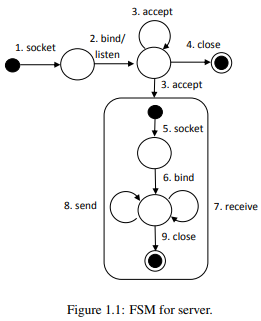
\includegraphics[width=.45\linewidth]{chap1_2.png} 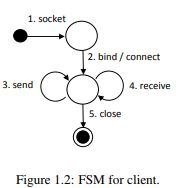
\includegraphics[width=.45\linewidth]{chap1_3.png}
$accept$ is \lstinline{while loop}, detail in rectangle: create a new socket (and therad) for commu. with client
\rtext{Simple protocol design}  complex number as string: $c_i = (a, b)$, $op \in \{add, sub, mul, div\}$,
C to S message format: $m_1 \textless c_1;c_2;op \textgreater$,
Status: $st \in \{ OK,msgIncomplete, ... \}$,
S to C message format: $m_2 \textless C_r; st \textgreater$
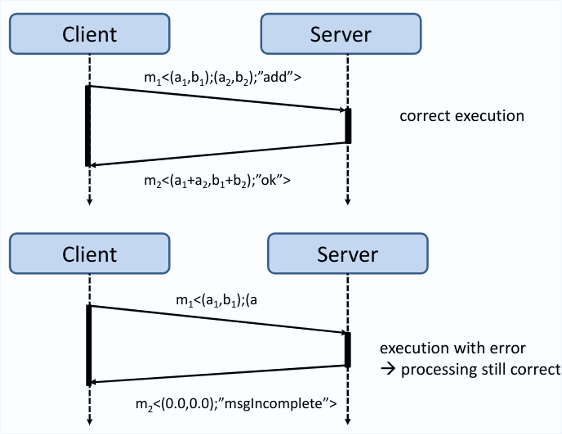
\includegraphics[width=.45\linewidth]{chap1_4.png} 

% TODO: code about socket clien server